% Chapter 4

\chapter{Proposed Methodology} % Main chapter title

\label{Chapter4} % For referencing the chapter elsewhere, use \ref{Chapter1} 

\lhead{Chapter 4. \emph{Proposed Methodology}} % This is for the header on each page - perhaps a shortened title

%------------------------
---------------------------------------------------------------

\section{CondLaneNet}

Given an input image I $\in$  {$R^{C \times H \times W}$}, the goal of our 
CondLaneNet is to predict a collection of lanes L = {$l_1$ , $l_2$ , ..., $l_N$}, 
where N is the total number of lanes. Generally, each lane $l_k$ is represented by an ordered set of coordinates as follows.
\begin{equation}
l_k = [(x_{k1} , y_{k1} ), (x_{k2} , y_{k2} ), ..., (x_{kN_k} , y_{kN_k} )]
\label{eqn:Einstein}
\end{equation}
 Where k is the index of lane and $N_k$ is the max number of sample points of the $k^{th}$ lane.
 
We describe a conditional lane detection method based on conditional convolution, which is a convolution operation with adjustable kernel parameters that focuses on instance-level discrimination abilities. The conditional detection method consists of two steps: instance detection and shape prediction. The instance detection stage predicts the object instance and regresses a set of dynamic kernel parameters for each instance. In the shape prediction step, conditional convolutions are utilized to determine the instance shape. The dynamic kernel settings are used in this method. Because each instance corresponds to a set of dynamic kernel parameters, shapes may be predicted instance by instance. Our conditional lane
detection strategy improves shape prediction and instance
detection to address the above problems.
\begin{figure}[htbp]
	\centering
		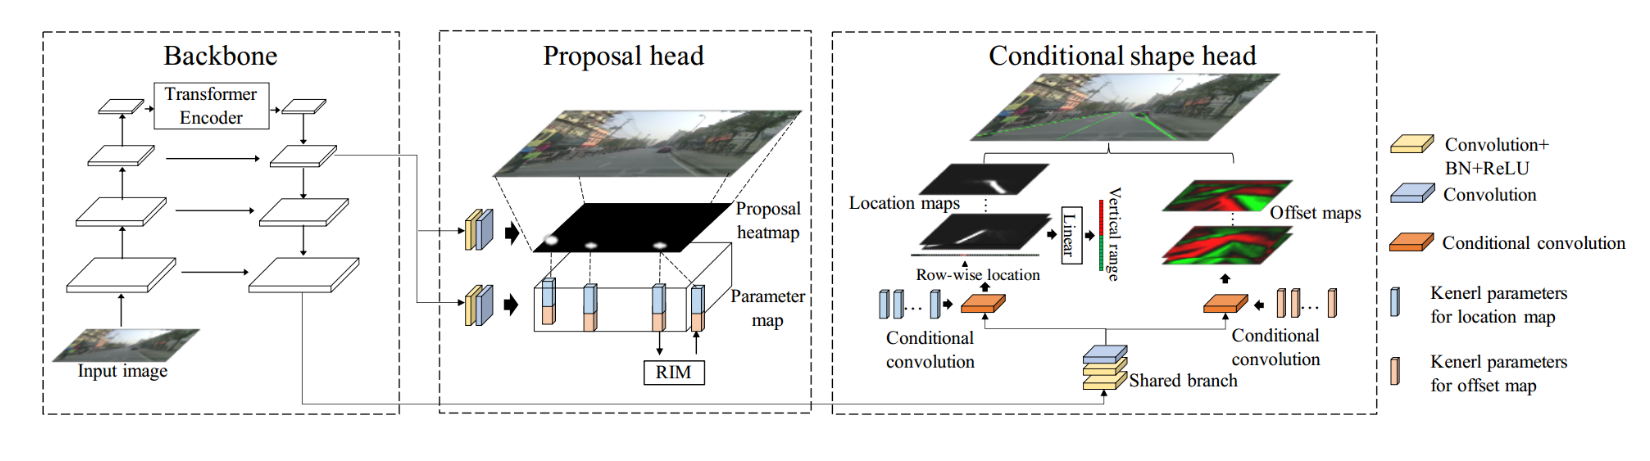
\includegraphics[scale=0.3]{Figures/condlane.png}
		\rule{35em}{0.5pt}
	\caption[CondLaneNet Architecture]{The CondLaneNet Architecture.}
	\label{fig:CondLaneNet Architecture}
\end{figure}

Figure 2 shows how we update the row-wise formulation [30] to estimate the line shape based on our conditional shape head. Based on the previous of the line shape, we estimate the lane position on each row and then aggregate the locations to produce the lane line in the order from bottom to top. Our row-wise formulation is made up of three parts: the row-wise location, the vertical range, and the offset map. Most row-wise detection algorithms rely on the first two outputs. In addition, we anticipate an offset map as the third output for additional tuning.

Each row on the location map includes an abscissa indicating the position of the lane line.
A basic way for obtaining row-wise location is to process the X-classes categorization in each row. The row-wise location is found in inference time by selecting the most responsive abscissa in each row. However, it is usual for the line to be located between the two grids, and both grids should have a strong response. To address this issue, we propose the following formulation.
We anticipate the likelihood of the lane line appearing in each grid for each row.

\begin{equation}
p_i = softmax(f^i_loc)
\label{eqn:Softmax Function}
\end{equation}

Where \emph{i} represents the \emph{ith}, is the feature vector of the \emph{ith} row of location map $f_loc$ , \emph{$p_i$} is the probability vector for the \emph{ith} row. The final row-wise location is defined as the expected abscissa.

\begin{equation}
E(x _i) = \sum_{j} j \times p_{ij}
\label{eqn:Softmax Function}
\end{equation}

Where \emph{E($x_i$)} is the expected abscissa, \emph{$p_{ij}$} is the probability of the lane line passing through the coordinate \emph{(j, i)}.

In the training phase, L1-loss is applied.

The vertical lane range is determined by
row-wisely predicting whether the lane line passes through
the current row, as is shown in Figure 4. We add a linear
layer and perform binary-classification row by row. We use
the feature vector of each row in the location map as the
input. The softmax-cross-entropy loss is adopted to guide
the training process.

\begin{equation}
E(x _i) = \sum_{j} j \times p_{ij}
\label{eqn:Softmax Function}
\end{equation}


\begin{figure}[htbp]
	\centering
		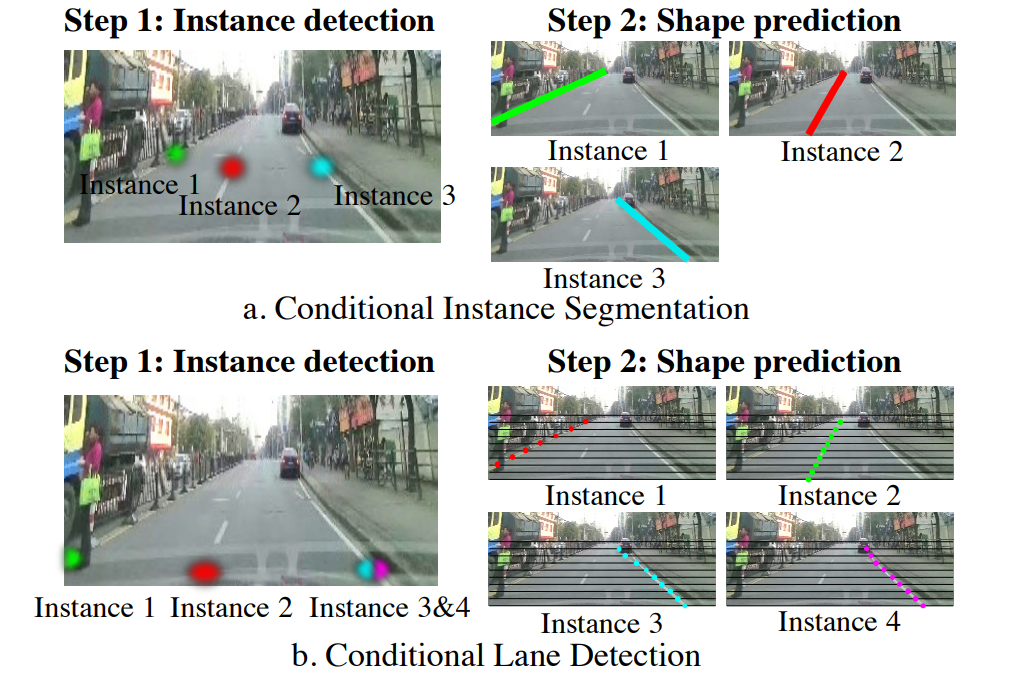
\includegraphics[scale=0.4]{Figures/condlaneprocess.png}
		\rule{35em}{0.5pt}
	\caption[The CondLaneNet Lane detection Process]{The CondLaneNet Lane detection process.}
	\label{fig:The CondLaneNet Lane Detection Process}
\end{figure}

The row-wise location defined in Equation 3
points to the abscissa of the vertex on the left side of the
grid, rather than the precise location. Thus, we add the off-
set map to predict the offset in the horizontal direction near
the row-wise location for each row.


We design the proposal head for instance detection, as is
shown in Figure 2. For general conditional instance seg-
mentation methods [35, 38], the instance is detected in anend-to-end pipeline by predicting the central of each object.
However, it is hard to predict the central for the slender and
curved lines because the visual characteristic of the line cen-
tral is not obvious.
We detect the lane instance by detecting the proposal
point located at the start point of the line. The start point has
a more clear definition and more obvious visual character-
istic than the central. We follow CenterNet [5] and predict
a proposal heatmap to detect the proposal points.


In the proposal head described above, each proposal
point is bound to a lane instance. However, in practice, mul-
tiple lane lines can fall in the same proposal point such as
the fork lanes. To deal with the above cases, we propose the
Recurrent Instance Module(RIM).

he structure of the proposed RIM is shown in Figure 5.
Based on LSTM(Long Short-term Memory) [9], the RIM
recurrently predicts a state vector s i and a kernel parame-
ter vector k i . We define s i as two-dimensional logits that
indicate two states: “continue” or “stop”. The vector k i
contains the kernel parameters for subsequent instance-wise
dynamic convolution. In the inference phase, the RIM re-
currently predicts the lane-wise kernel parameters bound to
the same proposal point until the state is “stop”.

he overall architecture is shown in Figure 2. We adopt
ResNet [8] as the backbone and add a standard FPN [23]
module to provide integrated multi-scale features. The pro-
posal head detects the lane instances by predicting the pro-
posal heatmap of shape 1 × H p × W p . Meanwhile, a pa-
rameter map of shape C p × H p × W p that contains the
dynamic kernel parameters is predicted. For the instance
with the proposal point located at (x p , y p ), the correspond-
ing dynamic kernel parameters are contained in the C p di-
mensional kernel feature vector at (x p , y p ) on the parameter
map. Further, given the kernel feature vector, the RIM re-
currently predicts the dynamic kernel parameters. Finally,
the conditional shape head predicts the line shape instance-
wisely conditioned on the dynamic kernel parameters.

Our framework requires a strong capability of context
feature fusion. For example, the prediction of the proposal
point is based on the features of the entire lane line whichgenerally has an elongated shape and long-range. There-
fore, we add a transformer encoder structure to the last layer
of the backbone for the fusion of contextual information.
We retain the two-dimensional spatial features in the en-
coder layer and use convolutions for feature extraction. The
structure of the transformer encoder used in our framework
is shown in Figure 6.

\section{ERFNet Model}

In this section, we introduce our efficient architecture for
real-time semantic segmentation. Our proposal aims at solving
an efficiency limitation that is inherently present in commonly
adopted versions of the residual layer, which is used in several
recent ConvNets that achieve top accuracy in classification [6]
and segmentation tasks [8][20][11]. By solving this limitation,
we manage to develop a semantic segmentation architecture
that makes a much more efficient use of parameters compared
to existing architectures, allowing our network to obtain a very
high segmentation accuracy while keeping top efficiency in
order to satisfy the constraints present in IV applications.

\begin{figure}[htbp]
	\centering
		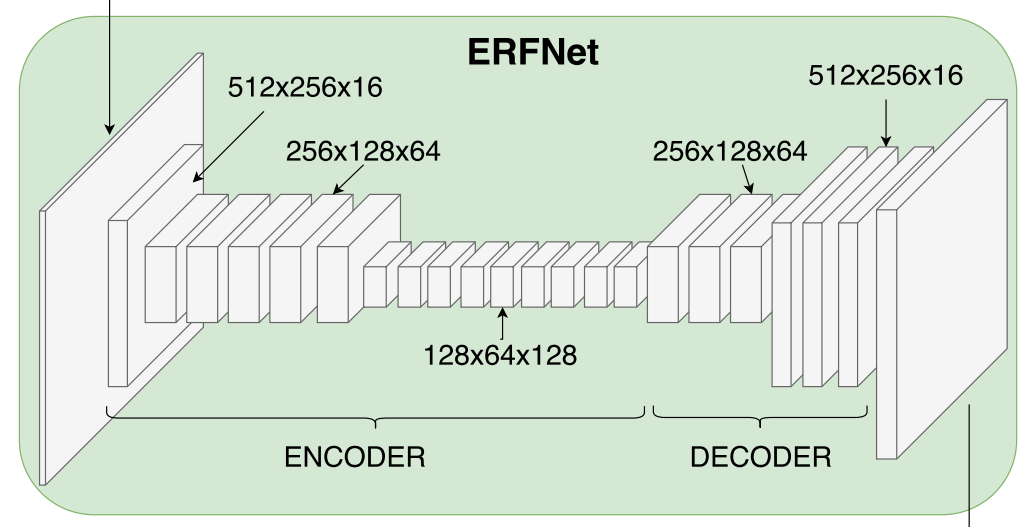
\includegraphics[scale=0.4]{Figures/erfnet.png}
		\rule{35em}{0.5pt}
	\caption[The ERFNet Model Architecture]{The ERFNet Model Architecture.}
	\label{fig:The ERFNet Model Architecture}
\end{figure}
Residual layers [6] have the property of allowing convolu-
tional layers to approximate residual functions, as the output
vector y of a layer vector input x becomes:
y = F(x, {W i }) + W s x
(1)
where W s is usually an identity mapping and F(x, {W i })
represents the residual mapping to be learned. This residual
formulation facilitates learning and significantly reduces the
degradation problem present in architectures that stack a large
amount of layers [6]. The original work proposes two instances
of this residual layer: the non-bottleneck design with two 3x3
convolutions as depicted in Fig. 2 (a), or the bottleneck version
as depicted in Fig. 2 (b). Both versions have similar number
of parameters and almost equivalent accuracy. However, the
bottleneck requires less computational resources and these
scale in a more economical way as depth increases. Hence, the
bottleneck design has been commonly adopted in state-of-the-
art networks [6][8][20][11]. However, it has been reported that
non-bottleneck ResNets gain more accuracy from increased
depth than the bottleneck versions, which indicates that they
are not entirely equivalent and that the bottleneck design still
suffers from the degradation problem [6][7][21].
We propose to redesign the non-bottleneck residual module
in a more optimal way by entirely using convolutions with 1D
filters (Fig. 2 (c)). As demonstrated in [22], any 2D filter can
be represented by a combination of 1D filters in the following
h
v
way. Let W $\in$ R C×d ×d ×F denote the weights of a typical
2D convolutional layer, where C is the number of input
planes, F is the number of output planes (feature maps) and
d h ×d v represents the kernel size of each feature map (typically
d h $\equiv$ d v $\equiv$ d). Let b $\in$ R F be the vector representing
h
v
the bias term for each filter and f i $\in$ R d ×d represent the
ith kernel in the layer. Common approaches first learn these
filters from data and then find low-rank approximations as
a post-processing step [23]. However, this approach requires
additional fine tuning and the resulting filters may not be
separable. Instead, [24] demonstrates that it is possible to relax
the rank-1 constraint and essentially rewrite f i as a linear
combination of 1D filters:

Considering an equal kernel size d for simplicity, it is trivial
to see that the decomposition reduces W 2D$\in$R C×d×d×F
of any 2D convolution into a pair of W 1D$\in$R C×d×F ,
resulting the equivalent dimensions of each 1D pair in dim =
2 × (C × d × F ). Therefore, this factorization can be ap-
plied to reduce the 3x3 convolutions on the original residual
modules. While larger filters would be more benefited by
this decomposition, applying it on 3x3 convolutions already
yields a 33\% reduction in parameters and further increases its
computational efficiency.
By leveraging this decomposition, we propose a new imple-
mentation of the residual layer that makes use of the described
1D factorization to accelerate and reduce the parameters of the
original non-bottleneck layer. We refer to this proposed mod-
ule as “non-bottleneck-1D” (non-bt-1D), which is depicted in
Fig. 2 (c). This module is faster (as in computation time)
and has less parameters than the bottleneck design, while
keeping a learning capacity and accuracy equivalent to the
non-bottleneck one. Table I summarizes the total dimensions
of the weights on the convolutions of every residual block,
comparing original ones with our proposed 1D factorizations.
Both non-bottleneck and bottleneck implementations can be
factorized into 1D kernels. However, the non-bottleneck design
is clearly more benefited, by receiving a direct 33\% reduction
in both convolutions and greatly accelerating its execution
time. As demonstrated in our experiments, this acceleration
even makes it faster than the bottleneck design, whose original
purpose according to [6] was to accelerate training time.

n this work, our main motivation is to obtain an architecture
that gets the best possible trade-off between accuracy and
efficiency. With this target in mind, we followed the current
trend of using convolutions with residual connections as the
core elements of our architecture, in order to leverage their
success in classification and segmentation problems. However,
as stated in the previous section, the commonly used residual
layers inherited some limitations in terms of learning capacity
and efficiency, which we aimed to minimize with our proposed
non-bottleneck-1D (non-bt-1D) layer. This novel block, that
leverages residual connections with factorized convolutions
and combines the strengths of bottleneck and non-bottleneck
designs, is the core of our architecture. Our network is de-
signed by stacking sequentially the proposed non-bt-1D layers
in a way that best leverages their learning performance and
efficiency.
Our architecture is fully depicted in Table II. We follow an
encoder-decoder architecture like SegNet [16] and ENet [11].
Contrary to architectures like FCN [5], where feature maps
from different layers need to be fused to obtain a fine-grain
output, our approach follows a more sequential architecture
based on an encoder segment producing downsampled feature
maps and a subsequent decoder segment that upsamples the
feature maps to match input resolution. Long-range skip
connections between the encoder and the decoder have been
used to improve accuracy in other works like [26]. However,
our architecture does not include these long-range skip connec-
tions as we did not obtain any empirical improvement. Fig. 1
contains a depiction of the feature maps generated by each of
the blocks in our architecture, from the RGB image (encoder’s
input) to the pixel class probabilities (decoder’s output).
The layers from 1 to 16 in our architecture form the encoder,
composed of residual blocks and downsampling blocks. Down-
sampling (reducing the spatial resolution) has the drawback
of reducing the pixel precision (coarser outputs), but it also
has two benefits: it lets the deeper layers gather more context
(to improve classification) and it helps to reduce computation.
Therefore, to keep a good balance we perform three downsam-
plings: at layers 1, 2 and 8. Our downsampler block, inspired
by the initial block of ENet [11], performs downsampling by
concatenating the parallel outputs of a single 3x3 convolution with stride 2 and a Max-Pooling module. ENet uses it only
as the initial block to perform early downsampling, but we
use it in all the downsampling layers that are present in
our architecture. Additionally, we also interleave some dilated
convolutions [27] in our non-bt-1D layers to gather more
context, which led to an improvement in accuracy in our
experiments. This technique has been proven more effective
(in terms of computational cost and parameters) than using
larger kernel sizes. In Table II, for those blocks that are
marked as “dilated”, we change the second pair of 3x1 and
1x3 convolutions for a pair of dilated 1D convolutions. We
also include Dropout [28] in all our non-bt-1D layers as a
regularization measure, although we triplicate its probability
(0.3 in contrast to 0.1 used in ENet), as this yielded better
results in our architecture.
The decoder segment is composed of the layers from 17
to 23. Its main task is to upsample the encoder’s feature
maps to match the input resolution. While SegNet had a
relatively symmetric encoder-decoder shape (i.e. decoder of
equal size to encoder), we follow a similar strategy to ENet
in having a small decoder whose only purpose is to upsample
the encoder’s output by fine-tuning the details. In contrast to
SegNet and ENet, we do not use max-unpooling operation
for the upsampling. Instead, our architecture includes simple
deconvolution layers with stride 2 (also known as transposed
convolutions or full-convolutions). The main advantage of
using deconvolutions is not requiring to share the pooling
indexes from the encoder. Therefore, deconvolutions simplify
memory and computation requirements. In addition, we em-
pirically obtained similar (or slightly better) accuracy.
\section{ERF-CondLaneNet}